\documentclass[11pt]{article}
\usepackage{graphicx} % For including images 
\usepackage{amsmath} % For advanced math formatting 
\usepackage{array} % For more flexible table formatting 
\usepackage{caption} % For customizing captions 
\usepackage{geometry} % For setting document margins 
\usepackage{float} % For controlling figure and table placement 
\geometry{margin=1in} % Set margins to 1 inch 
\usepackage{xepersian} % Package for Persian language support with XeLaTeX 


\settextfont{Arial}        

\title{استفاده از الگوریتم ژنتیک برای حل یک معادله ساده ریاضی}
\author{دنی هرماوانتو\\موسسه علوم اندونزی\\آدرس پست الکترونیکی:
\href{denny.hermawanto@gmail.com} }


\date{\today}

\begin{document}

\maketitle

%%%%%%%%%%%%%%%%%%%%%%%%
%%%%%%%%%%%%%%%%%%%%%%%%
\section{چكيده}
\textbf{این مطلب استفاده از الگوریتم ژنتیک را به شکلی ساده به همراه مثال برای افراد مبتدی شرح میدهد. ابتدا فلسفه اساسی و فلوچارت این الگوریتم شرح داده می‌شود و در مرحله بعد محاسبات قدم به قدم الگوریتم ژنتیک برای حل یک مسأله ساده تساوی ریاضیات بصورت کامل شرح داده می‌شود.}

%%%%%%%%%%%%%%%%%%%%%%%%
%%%%%%%%%%%%%%%%%%%%%%%%
\section{فلسفه پایه الگوریتم‌های ژنتیک}
توسعه و گسترش یافت که الهام گرفته از تئوری تکامل داروین است. مبنای این نظریه هم بقای گونه‌ها بر اساس میزان ارزش آن‌هاست. هر چه قوی‌تر احتمال بقا هم بیشتر است. داروین همچنین معتقد است که بقای یک نسل میتواند بوسیله فرآیند تولید مثل، انتخاب، برش و جهش حفظ شود. بعدها از ایده داروین در خصوص تکامل برای بدست آوردن راه‌حل بهینه در مسائل محاسباتی استفاده شد که یکی از معروف‌ترین این الگوریتم‌ها، الگوریتم ژنتیک است.

راه‌حل‌هایی که توسط الگوریتم‌های ژنتیک تولید می‌شود یک کروموزوم نامیده می‌شود و مجموعه‌ای از کروموزم‌ها، جمعیت (population) نامیده می‌شوند. کروموزم‌ها از ژن‌ها تشکیل شده‌اند و مقدار آن‌ها می‌تواند عددی دودویی، سمبل‌ها یا کاراکترها باشد که وابسته به مسأله‌ای است که قصد حل نمودن آن را داریم. شایان ذکر است نحوه نمایش کروموزوم‌ها و مقادیر آن‌ها یکی از اساسی‌ترین قسمت‌های حل یک مسأله با استفاده از الگوریتم ژنتیک است و دیگر قسمت بسیار مهم در این الگوریتم‌ها تعریف تابع برازش است که در قسمت بعدی به آن پرداخته می‌شود.

ارزش و بهای هر کروموزوم توسط تابعی تحت نام برازش اندازه‌گیری می‌شود. در واقع تابع برازش میزان مفید و مناسب بودن راه‌حل برای مسأله مورد نظر را اندازه‌گیری می‌نماید. پس از هر مرحله‌ای که الگوریتم ژنتیک تکرار شد، برازش هر یک از راه‌حل‌های تولید شده (کروموزوم‌ها) اندازه‌گیری می‌شود. برخی از کروموزم‌ها درون جمعیت تحت فرآیندی به نام crossover با یکدیگر ترکیب می‌شوند و بدین صورت کروموزوم‌های جدیدی که فرزند نامیده می‌شود تولید می‌کنند که ترکیب ژن این کروموزم‌های جدید ترکیبی از ژن‌های والدین آن‌هاست. در یک نسل تعدادی از کروموزوم‌ها نیز در ژن‌های خود دچار جهش (mutation) می‌شوند.

تعداد کروموزوم‌هایی که تحت تأثیر crossover و جهش قرار می‌گیرند بوسیله نرخ برش و نرخ جهش کنترل می‌شوند. کروموزومی در جمعیت که برای نسل بعدی حفظ و نگاهداری می‌شود بوسیله قانون تکامل داروین انتخاب می‌شود. کروموزومی که مقدار برازش بالاتری دارد از احتمال بالاتری برای انتخاب دوباره در نسل بعدی برخوردار است. بعد از چندین نسل، مقدار کروموزم به یک مقدار خاص که بهترین راه‌حل برای مسأله است همگرا می‌شود.

%%%%%%%%%%%%%%%%%%%%%%%%
%%%%%%%%%%%%%%%%%%%%%%%%
\section{مراحل الگوریتم ژنتیک}

در الگوریتم ژنتیک فرآیند به شرح ذیل است:
\begin{enumerate}
    \item تعداد کروموزوم‌ها، نسل‌ها و نرخ جهش و نرخ برش معین می‌شود.
    \item بر اساس تعداد جمعیت کروموزوم - کروموزوم ایجاد می‌شود و ژن‌های کروموزوم - با یک مقدار تصادفی مقدار دهی اولیه می‌شوند.
    \item قدم‌های 3 تا 8 را تا زمانی که تعداد نسل‌ها برآورده شود انجام می‌شود.
    \item مقدار برازش کروموزوم بوسیله محاسبه تابع هدف (objective function) مورد ارزیابی قرار می‌گیرد.
    \item انتخاب کروموزوم.
    \item برش.
    \item جهش.
    \item کروموزم جدید (فرزند).
    \item راه‌حل بهترین کروموزوم‌ها.
\end{enumerate}
\\
\\
فلوچارت الگوریتم را میتوان در شکل زیر مشاهده نمود:

\begin{figure}[h]
    \centerline{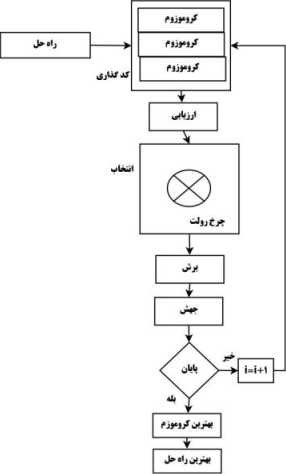
\includegraphics[scale=1.5]{picture.jpg}}
    \caption{نمودار جریان الگوریتم ژنتیک}
    \label{fig}
\end{figure}

%%%%%%%%%%%%%%%%%%%%%%%%
%%%%%%%%%%%%%%%%%%%%%%%%
\section*{مثال عددی}
در اینجا یک مثال از کاربردی که از الگوریتم ژنتیک برای حل یک مسئله ترکیبی استفاده می‌کند را توضیح می‌دهیم. فرض کنیم که تساوی زیر را داریم:
 \[ a + 2b + 3c + 4d = 30 \] 
 
 از الگوریتم ژنتیک برای بدست آوردن مقادیر \(a\)، \(b\)، \(c\) و \(d\) برای حل تساوی ذکر شده استفاده کنیم. در ابتدا باید تابع هدف را فرموله کنیم. برای این مسئله هدف مینیمم نمودن مقدار تابع \( F(X) \) جایی که:

 \[ F(X) = \left| a + 2b + 3c + 4d - 30 \right| \] 
 
 از آنجا که چهار متغیر در تساوی وجود دارد، یعنی \(a\)، \(b\)، \(c\)، \(d\)، می‌توانیم کروموزوم‌ها را به صورت زیر شکل دهیم:

 \[ \begin{array}{cccc} d & c & b & a \\ \end{array} \]  
 
 برای افزودن سرعت محاسبات، می‌توانیم مقدار متغیرها را به اعداد صحیح بین 0 تا 30 محدود نماییم. 
 
 %%%%%%%%%%%%%%%%%%%%%%%%
 \textbf{قدم اول: مقداردهی اولیه}


  برای نمونه، تعداد کروموزوم‌ها درون جمعیت را عدد 6 تعریف می‌کنیم. سپس مقادیر تصادفی را برای ژن‌هایی که تشکیل دهنده کروموزوم مورد نظر ما هستند تولید می‌کنیم. پس همانطور که ملاحظه می‌شود، 6 کروموزومی را که در اختیار داریم به صورت زیر با اعداد تصادفی مقداردهی می‌نماییم:
 
 \\
\[
\begin{align*}
\text{Chromosome[1]} & = [a; b; c; d] = [12; 05; 23; 08] \\ \text{Chromosome[2]} & = [a; b; c; d] = [03; 21; 18; 03] \\ \text{Chromosome[3]} & = [a; b; c; d] = [10; 04; 13; 14] \\ \text{Chromosome[4]} & = [a; b; c; d] = [20; 01; 10; 06] \\ \text{Chromosome[5]} & = [a; b; c; d] = [01; 04; 13; 19] \\ \text{Chromosome[6]} & = [a; b; c; d] = [20; 05; 17; 01] \\ 
\end{align*}
\]
\\
%%%%%%%%%%%%%%%%%%%%%%%% 
\textbf{قدم دوم: ارزیابی راه‌حل‌ها (کروموزوم‌ها)}
 
  در این مرحله مقدار تابع هدف برای هر کروموزومی که در مرحله مقداردهی جمعیت اولیه تولید شده است، محاسبه می‌شود: 

\[
\begin{align*}
F\_obj[1] &= \text{Abs}\left(( 12 + 2 \times 05 + 3 \times 23 + 4 \times 08 ) - 30\right) \\ 
&= \text{Abs}\left((12 + 10 + 69 + 32) - 30\right) \\ 
&= \text{Abs}(123 - 30) \\ &= 93 \\ 
\\
F\_obj[2] 
&= \text{Abs}\left((02 + 2 \times 21 + 3 \times 18 + 4 \times 03) - 30\right) \\ 
&= \text{Abs}\left((02 + 42 + 54 + 12) - 30\right) \\ 
&= \text{Abs}(110 - 30) \\ &= 80 \\ 
\\ 
F\_obj[3] 
&= \text{Abs}\left((10 + 2 \times 04 + 3 \times 13 + 4 \times 14) - 30\right) \\ 
&= \text{Abs}\left((10 + 08 + 39 + 56) - 30\right) \\ 
&= \text{Abs}(113 - 30) \\ &= 83 \\ 
\\ 
F\_obj[4] &= \text{Abs}\left((20 + 2 \times 01 + 3 \times 10 + 4 \times 06) - 30\right) \\ 
&= \text{Abs}\left((20 + 02 + 30 + 24) - 30\right) \\ &= \text{Abs}(76 - 30) \\ 
&= 46 \\ 
\\ 
F\_obj[5] &= \text{Abs}\left((01 + 2 \times 04 + 3 \times 13 + 4 \times 19) - 30\right) \\ &= \text{Abs}\left((01 + 08 + 39 + 76) - 30\right) 
\\ 
&= \text{Abs}(124 - 30) \\ &= 94 \\ 
\\ 
F\_obj[6] 
&= \text{Abs}\left((20 + 2 \times 05 + 3 \times 17 + 4 \times 01) - 30\right) \\
&= \text{Abs}\left((20 + 10 + 51 + 04) - 30\right) \\ &= \text{Abs}(85 - 30) \\ 
&= 55 
\end{align*}
\]
%%%%%%%%%%%%%%%%%%%%%%%%
\textbf{ مرحله سوم: انتخاب}

با ارزشترین کروموزوم از شانس و احتمال بیشتری برای انتخاب شدن به منظور تولید نسل بعدی دارد. برای محاسبه احتمال برازش باید برازش هر کروموزوم محاسبه شود. برای جلوگیری از مشکل تقسیم بر صفر مقدار تابع هدفی که برای هر کروموزوم در مرحله قبل بدست آمد با عدد  ۱ جمع می‌شود: 

\\

\[
\begin{align*} 
\text{Fitness}[1] &= \frac{1}{1+F\_obj[1]} \\ 
&= \frac{1}{94} \\ 
&= 0.0106 \\ 
\\ 
\text{Fitness}[2] &= \frac{1}{1+F\_obj[2]} \\ 
&= \frac{1}{81} \\ 
&= 0.0123 \\ 
\\ 
\text{Fitness}[3] &= \frac{1}{1+F\_obj[3]} \\
&= \frac{1}{84} \\ 
&= 0.0119 \\ 
\\ 
\text{Fitness}[4] &= \frac{1}{1+F\_obj[4]} \\ 
&= \frac{1}{47} \\ 
&= 0.0213 \\ 
\\
\text{Fitness}[5] &= \frac{1}{1+F\_obj[5]} \\  
&= \frac{1}{95} \\ 
&= 0.0105 \\ 
\\ 
\text{Fitness}[6] &= \frac{1}{1+F\_obj[6]} \\ 
&= \frac{1}{56} \\ 
&= 0.0179 \\
\end{align*}
\]


\[
Total=0.0106+0.0123+0.0119+0.0213+0.0105+0.0179=0.0845
\]
%%%%%%%%%%%%%%%%%%%%%%%%

احتمال مربوط به هر کروموزوم را بوسیله فرمول 
$P[i] = \text{Fitness}[i] / \text{Total}$
 محاسبه می‌نماییم:
 
 \\
 \[
\begin{align*}
\text{P}[1] &= \frac{0.0106}{0.0845}\\
&=0.1254\\
\\
\text{P}[2] &= \frac{0.0123}{0.0845}\\
&=0.1456\\
\\
\text{P}[3] &=\frac{0.0119}{0.0845}\\
&=0.1408\\
\\
\text{P}[4] &=\frac{0.0213}{0.0845}\\
&=0.2521\\
\\
\text{P}[5] &=\frac{0.0105}{0.0845}\\
&=0.1243\\
\\
\text{P}[6] &= \frac{0.0179}{0.0845}\\
&=0.2118\\
\\
\end{align*}
\]

با توجه به احتمالاتی که در بالا محاسبه شده است، مشاهده می‌شود که کروموزوم ۴ بیشترین برازش را دارا می‌باشد و بنابراین احتمال انتخاب آن برای نسل بعدی کروموزوم‌ها بسیار بالا است. برای فرایند انتخاب از روش جرخ رولت استفاده می‌کنیم که بدین منظور ابتدا باید مقادیر احتمال تجمعی (\lr{cumulative probability}) را محاسبه کنیم: 
\[
\begin{align*} 
\text{C}[1] &= 0.1254 \\ 
\text{C}[2] &= 0.1254 + 0.1456 = 0.2710 \\ 
\text{C}[3] &= 0.1254 + 0.1456 + 0.1408 = 0.4118 \\ 
\text{C}[4] &= 0.1254 + 0.1456 + 0.1408 + 0.2521 = 0.6639 \\ 
\text{C}[5] &= 0.1254 + 0.1456 + 0.1408 + 0.2521 + 0.1243 = 0.7882 \\ 
\text{C}[6] &= 0.1254 + 0.1456 + 0.1408 + 0.2521 + 0.1243 + 0.2118 = 1.0\\ \end{align*}
\]
با داشتن مقادیر احتمال تجمعی استفاده از چرخ رولت در فرآیند انتخاب امکان پذیر می گردد. فرآیند بعدی تولید یک عدد تصادفی در محدوده ۰ تا ۱ است که آن را R  می‌نامیم: 

\\

\[
\begin{align*}
\text{R}[1] &= 0.201\\ 
\text{R}[2] &= 0.284\\
\text{R}[3] &= 0.099\\ 
\text{R}[4] &= 0.822\\ 
\text{R}[5] &= 0.398\\
\text{R}[6] &= 0.501 
\end{align*}
\]
\\
\\
اگر برای مثال عدد تصادفی \( R[1] \)  بزرگتر از \( C[1] \)  و کوچکتر از  \( C[2] \) بود در این صورت \( \text{Chromosome}[2] \)  به عنوان یک کروموزوم در جمعیت جدید برای تولید نسل بعدی مورد استفاده قرار می‌گیرد. با توجه به مقادیر نمونه‌های بالا خواهیم داشت:
\\
\[
\begin{align*}
\text{NewChromosome}[1] &= \text{Chromosome}[2] \\
\text{NewChromosome}[2] &= \text{Chromosome}[3] \\
\text{NewChromosome}[3] &= \text{Chromosome}[1] \\
\text{NewChromosome}[4] &= \text{Chromosome}[6] \\
\text{NewChromosome}[5] &= \text{Chromosome}[3] \\
\text{NewChromosome}[6] &= \text{Chromosome}[4]
\end{align*}
\]
\\
\\

و کروموزوم ها در جمعیت به صورت زیر خواهد شد:
\\
\[
\begin{align*}
\text{Chromosome}[1] &= [02;21;18;03] \\
\text{Chromosome}[2] &= [10;04;13;14] \\
\text{Chromosome}[3] &= [12;05;23;08] \\
\text{Chromosome}[4] &= [20;05;17;01] \\
\text{Chromosome}[5] &= [10;04;13;14] \\
\text{Chromosome}[6] &= [20;01;10;06]
\end{align*}
\]
\\
\\

\textbf{مرحله ۴: برش\(crossover\)}

در این مثال از برش یک نقطه ای (\text{one cut point})\ استفاده می‌نماییم. به صورت تصادفی یک محل در کروموزوم والدین انتخاب شده و سپس زیر کروموزوم‌هایی که از این نقطه بدست آمده‌اند در دو واحد تعویض می‌شود. کروموزوم‌های والدینی که با همدیگر جفت شده‌اند به صورت تصادفی انتخاب می‌شوند و تعداد کروموزوم‌هایی که جفت می‌شوند توسط پارامتری به نام نرخ برش (\text{crossover rate ρc})\ معین می‌شود. شبه کد فرآیند برش در ذیل آورده شده است:
\begin{flushleft}
\begin{verbatim}
begin 
       k← 0;
       while(k<population) do 
       R[k] = random(0-1); 
       if(R[k]< ρc) then
select Chromosome[k] as parent; 
       end;
       k = k + 1;
       end;
end;
\end{verbatim}
\end{flushleft}


اگر $R[k] < \rho_c$ باشد کروموزوم $k$ به عنوان یکی از والدین انتخاب می‌شود. فرض کنیم که نرخ برش را $25\%$ در نظر گرفته باشیم، در این صورت کروموزوم شماره $k$ در صورتی برای برش انتخاب می‌شود اگر مقدار عدد تصادفی تولید شده برای کروموزوم $k$ کمتر از $0.25$ باشد. در فرایند را به صورت زیر ادامه می‌دهیم. ابتدا به تعداد جمعیتی که داریم عدد تصادفی $R$ تولید می‌نماییم:

\[
\begin{align*}
\text{R}[1] &= 0.191\\
\text{R}[2] &= 0.259\\
\text{R}[3] &= 0.760\\
\text{R}[4] &= 0.006\\
\text{R}[5] &= 0.159\\
\text{R}[6] &= 0.340\\
\end{align*}
\]
\\

با توجه به اعداد نمونه تصادفی که در بالا آورده شده است، والدین $\text{Chromosome}[1]$, $\text{Chromosome}[4]$ و $\text{Chromosome}[5]$ برای عملگر برش انتخاب می‌شوند. حالا با توجه این والدین ترکیب همه‌ی آن‌ها را بدست آوریم که به صورت زیر خواهد بود:


\begin{align*}
\text{Chromosome}[1]>< \text{ Chromosome}[4] \\
\text{Chromosome}[4]>< \text{ Chromosome}[5] \\
\text{Chromosome}[5]><\text{ Chromosome}[1]\\
\end{align*}

بعد از انتخاب کروموزوم‌ها برای برش، فرآیند بعدی مشخص نمودن محل نقطه برش است. این کار با تولید یک عدد تصادفی بین عدد ۱ تا طول کروموزوم انجام می‌شود. در مثال ما عدد تصادفی باید بین ۱ تا ۳ باشد. بعد از این که نقطه برش را بدست آوردیم، کروموزوم‌های والد در آن نقطه برش خورده و ژن‌های آن‌ها تعویض می‌شود و یک فرزند جدید تولید می‌شود. برای مثال ما سه عدد تصادفی زیر را تولید نمودیم:
\[ C[1] = 1 \]
\[ C[2] = 1 \]
\[ C[3] = 2 \]
\\
و کروموزوم‌ها به صورت زیر تحت تأثیر عملگر برش قرار می‌گیرند. همانگونه که مشاهده می‌شود ژن‌های والدین به ترتیب در ژن‌های شماره ۱، شماره ۱ و شماره ۲ برش داده می‌شوند:

\[
\begin{align*}
\text{Chromosome}[1] &= \text{Chromosome}[1] >< \text{Chromosome}[4] \\
&= [02;21;18;03] >< [20;05;17;01] \\
&= [02;05;17;01] \\
\text{Chromosome}[4] &= \text{Chromosome}[4] >< \text{Chromosome}[5] \\
&= [20;05;17;01] >< [10;04;13;14] \\
&= [20;04;13;14] \\
\text{Chromosome}[5] &= \text{Chromosome}[5] >< \text{Chromosome}[1] \\
&= [10;04;13;14] >< [02;21;18;03] \\
&= [10;04;18;03]
\end{align*}
\]
\\


بعد از انجام اولین فرآیند برش در الگوریتم ژنتیک مورد نظرمان، جمیعن ما به صورت زیر خواهد بود:

\[
\begin{align*}
\text{Chromosome}[1] &= [02;05;17;01] \\
\text{Chromosome}[2] &= [10;04;13;14] \\
\text{Chromosome}[3] &= [12;05;23;08] \\
\text{Chromosome}[4] &= [20;04;13;14] \\
\text{Chromosome}[5] &= [10;04;18;03] \\
\text{Chromosome}[6] &= [20;01;10;06]
\end{align*}
\]
\\
\\

\textbf{مرحله ۵: جهش }
تعداد کروموزوم هایی که جمعیت مورد جهش قرار می‌گیرند، توسط پارامتر نرخ جهش مشخص می‌شوند، با تعویض تصادفی مقدار یک ژن که در یک موقعیت تصادفی قرار دارد با مقدار جدید انجام می‌شود. برای انجام این فرایند مراحل زیر را انجام می‌دهیم. ابتدا باید مجموع کل ژن‌های موجود در جمعیت را محاسبه کنیم. در مثال ما از فرمول زیر بدست می‌آید:

تعداد کل ژن‌ها = تعداد ژن‌های هر کروموزوم * تعداد جمعیت = ۶ * ۴ = ۲۴

فرآیند جهش با تولید یک عدد تصادفی بین ۱ و تعداد کل ژن‌های (۱ تا ۲۴ در مثال ما) انجام می‌شود. اگر مقدار عدد تصادفی تولید شده کمتر از نرخ جهش (\texttt{mutation\_rate}) باشد، در این صورت موقعیت این ژن در کروموزوم نشان‌گذاری می‌شود. فرض کنیم که نرخ جهش را ۱۰٪ در نظر بگیریم، که در این صورت انتظار داریم که ۱۰٪ (۰.۱) کل ژن‌ها در جمعیت جهش داده شوند:
\\
\\
تعداد کل جهش‌ها = ۲۴ * ۰.۱ = ۲.۳ = ۲

حالا اگر فرض کنیم که اعداد تصادفی که تولید شده‌اند ۱۲ و ۱۸ باشند، در این صورت کروموزوم‌هایی که جهش دارند کروموزوم شماره ۳ در ژن شماره ۴ آن و کروموزوم شماره ۵ رد ژن شماره ۲ آن خواهند بود. مقدار ژن‌های جهش یافته در نقطه جهش بوسیله اعداد تصادفی بین ۰ تا ۳۰ عوض می‌شوند. اگر اعداد تصادفی تولید شده ۲ و ۵ باشند، سپس ترکیب کروموزوم‌ها بعد از جهش به صورت زیر است:

\[
\begin{array}{ll}
\text{Chromosome}[1] & = [02;05;17;01] \\
\text{Chromosome}[2] & = [10;04;13;14] \\
\text{Chromosome}[3] & = [12;05;23;02] \\
\text{Chromosome}[4] & = [20;04;13;14] \\
\text{Chromosome}[5] & = [10;05;18;03] \\
\text{Chromosome}[6] & = [20;01;10;06]
\end{array}
\]
\\
\\
بعد از پایان فرآیند جهش یک تکرار یا یک نسل از الگوریتم ژنتیک داریم که باید این نسل جدید را مجددا توسط تابع هدف مورد ارزیابی قرار دهیم که ارزیابی آن مانند آنچه قبلا گفته شد انجام می‌شود:
\[
\begin{array}{ll}
\text{Chromosome[1]} & = [02;05;17;01] \\
F_{\text{obj}[1]} & = \text{Abs}\left((02 + 2*05 + 3*17 + 4*01) - 30\right) \\
& = \text{Abs}\left((2 + 10 + 51 + 4) - 30\right) \\
& = \text{Abs}(67 - 30) \\
& = 37 \\
\text{Chromosome[2]} & = [10;04;13;14] \\
F_{\text{obj}[2]} & = \text{Abs}\left((10 + 2*04 + 3*13 + 4*14) - 30\right) \\
& = \text{Abs}\left((10 + 8 + 33 + 56) - 30\right) \\
& = \text{Abs}(107 - 30) \\
& = 77 \\
\text{Chromosome[3]} & = [12;05;23;02] \\
F_{\text{obj}[3]} & = \text{Abs}\left((12 + 2*05 + 3*23 + 4*02) - 30\right) \\
& = \text{Abs}\left((12 + 10 + 69 + 8) - 30\right) \\
& = \text{Abs}(87 - 30) \\
& = 47 \\
\text{Chromosome[4]} & = [20;04;13;14] \\
F_{\text{obj}[4]} & = \text{Abs}\left((20 + 2*04 + 3*13 + 4*14) - 30\right) \\
& = \text{Abs}\left((20 + 8 + 39 + 56) - 30\right) \\
& = \text{Abs}(123 - 30) \\
& = 93 \\
\text{Chromosome[5]} & = [10;05;18;03] \\
F_{\text{obj}[5]} & = \text{Abs}\left((10 + 2*05 + 3*18 + 4*03) - 30\right) \\
& = \text{Abs}\left((10 + 10 + 54 + 12) - 30\right) \\
& = \text{Abs}(86 - 30) \\
& = 56 \\
\text{Chromosome[6]} & = [20;01;10;06] \\
F_{\text{obj}[6]} & = \text{Abs}\left((20 + 2*01 + 3*10 + 4*06) - 30\right) \\
& = \text{Abs}\left((20 + 2 + 30 + 24) - 30\right) \\
& = \text{Abs}(76 - 30) \\
& = 46 \\
\end{array}
\]
\\
\\

همانگونه که از ارزیابی کروموزوم ها در جمعیت جدید مشاهده می‌شود تابع هدف کاهش یافته است که به این معناست که ما کروموزومها یا راه حل های بهتری نسبت به کروموزومهای نسل قبل داریم. بنابراین کروموزومها برای تکرار بعدی به صورت زیر خواهد بود:
\[
\begin{array}{ll}
\text{Chromosome}[1] & = [02;05;17;01] \\
\text{Chromosome}[2] & = [10;04;13;14] \\
\text{Chromosome}[3] & = [12;05;23;02] \\
\text{Chromosome}[4] & = [20;04;13;14] \\
\text{Chromosome}[5] & = [10;05;18;03] \\
\text{Chromosome}[6] & = [20;01;10;06]
\end{array}
\]
کروموزوم های جدید تحت تأثیر فرآیند مشابهی با انچه با نسل قبلی کروموزومها انجام شد قرار می‌گیرند. مثل ارزیابی، انتخاب، برش و جهش و  در پایان هر تکرار نیز نسل جدیدی از کروموزومها برای تکرار بعدی تولید می‌شود. این فرآیند تا رسیدن به تعداد تکرار های از پیش تعریف شده با بدست آمدن یک شرط ادامه می‌یابند. در این مثال حدوداً بعد از ۵۰ نسل بهترین کروموزوم بدست می‌آید:
\[
\text{Chromosome} = [07; 05; 03; 01]
\]
که بدان معناست که اگر این اعداد معادله این که در ابتدا داشتیم قرار دهیم خواهیم داشت:
\[ a + 2b + 3c + 4d = 30 \]
\[ 7 + (2 \times 5) + (3 \times 3) + (4 \times 1) = 30 \]
در این مثال ساده به خوبی کارایی و قدرت الگوریتم ژنتیک در حل مسائل بهینه سازی مشاهده می‌شود.

\end{document}